\chapter{Hardware Design and Development of an Integrated Mobile Platform}
\label{cha:Platform }


\begin{figure}
\centering
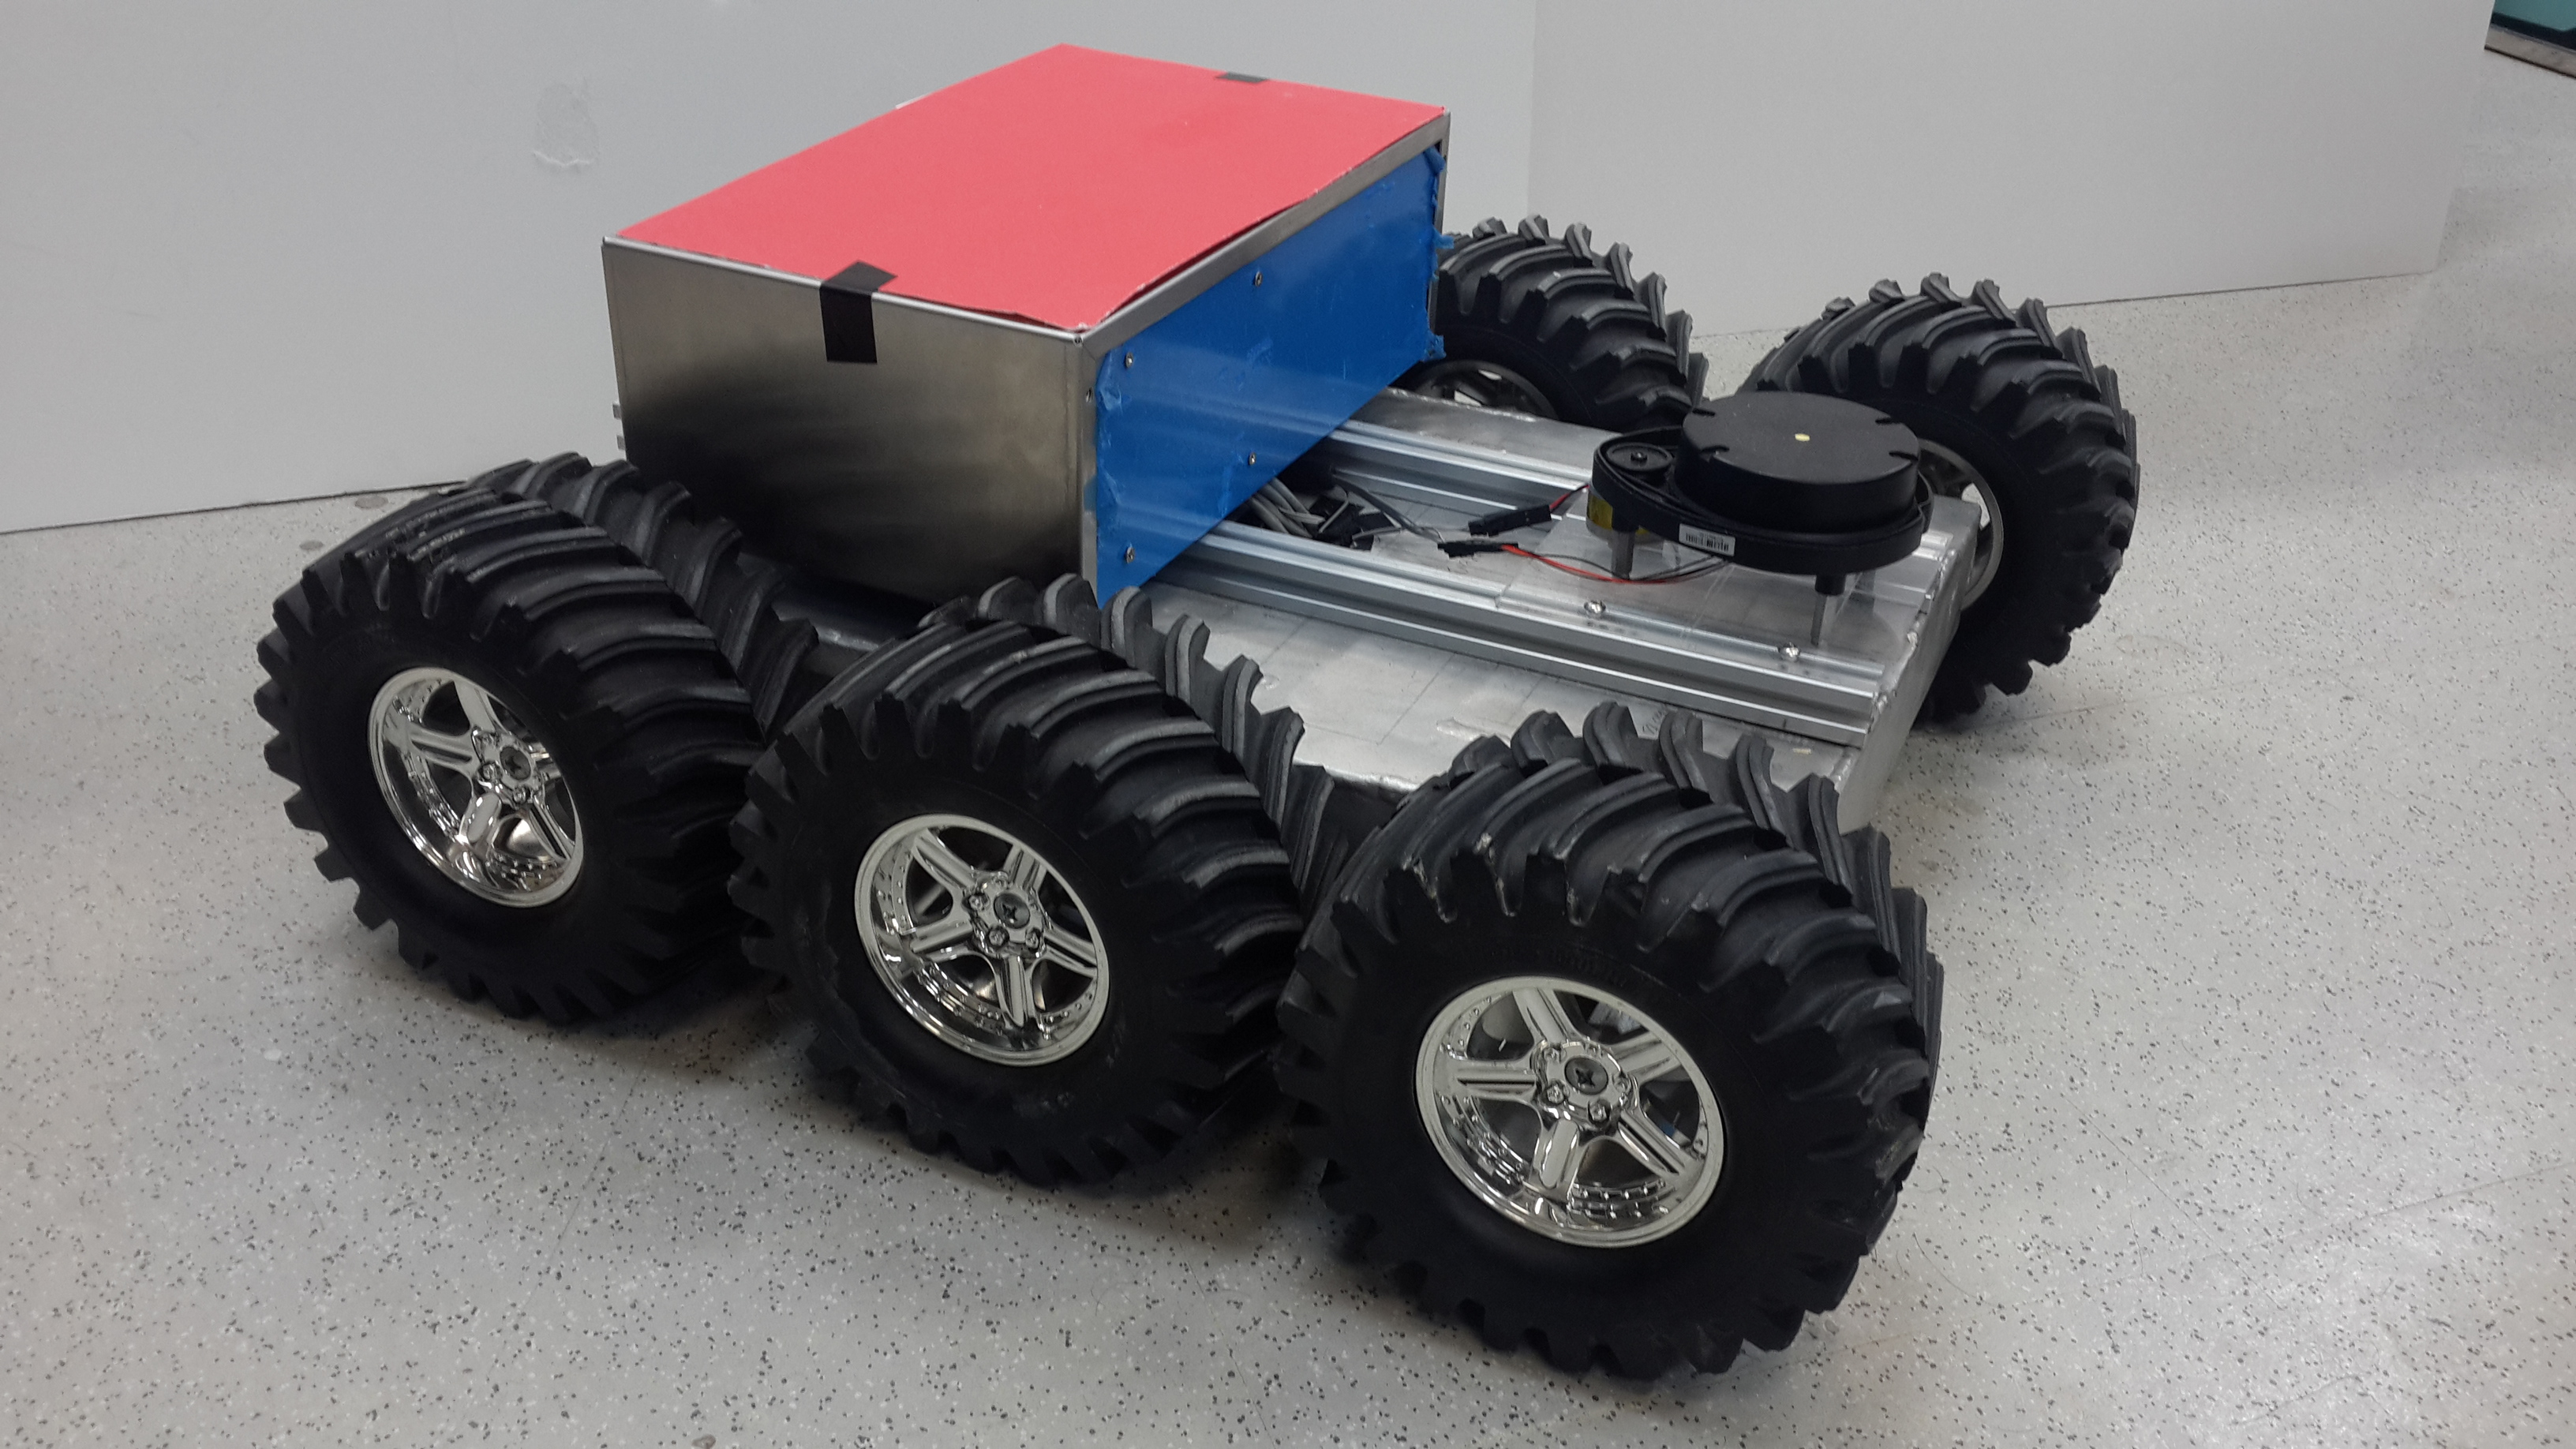
\includegraphics[width=0.5\textwidth]{IMP_color}
\caption{The Integrated Mobile Platform.}
\label{fig:IMP_color}
\end{figure}
\section{Overview and Design Goals}

The Integrated Mobile Platform (IMP) is designed as a robust, scalable platform for Simultaneous Localization and Mapping in a variety of complex environments along with capability for autonomous navigation and decision making. IMP is designed as a platform that can be used both for deployment as well as research. Hence, along with robustness, modularity is also emphasized in the design. It is a mobile robot which can be used either as an independent agent or as a long range mobilization unit in a cooperative team, requiring long range capability and considerable payload capacity.

For the primary purpose of SLAM, the major requirements of such a platform are:
\begin{description}
	\item[Movement] Has to be able to move with a variety of speeds and relatively small turning radii as it is to be used indoors. 
	\item[Self-position acknowledgment] Has to have proprioceptive sensors which give an estimate of it's own position and orientation.
	\item[Environment sensing] Has to have sensors to understand the environment. 
	\item[On-board computer] Has to have sufficient on-board processing power to do the computations necessary for SLAM.
	\item[Real time controller] Has to have a capability to implement real time control.
	\item[Communication] Has to have robust communication between the different components and also with the ground station. 
	\item[Memory] Has to have sufficient on-board memory to collect data to enable testing of SLAM algorithms off line.  
	\item[Flexibility] The various components both hardware and software need to be designed in such a way that it is easy to switch them around.
\end{description}

While these requirements define the bare minimum that is needed for such a platform, the design goals that guided the development of IMP were more broad. The design goals were as follows:

\begin{itemize}
	\item Have a hardware design capable of supporting large payloads and which can be scaled for any desired run time.
	\item Have enough computational power for implementing real time algorithms for autonomy.
	\item Design modular hardware and software interfaces for the sensors to allow testing of different sensors and sensor fusion algorithms.
\end{itemize}

With these goals in mind, IMP was designed as a six wheeled differential drive platform with a multi processor control system, including two micro-controllers and an on-board computer and equipped with a scanning laser range finder and monocular camera. 

The following section discusses the design process involved and the resulting features of IMP, first with respect to the hardware components. The next section discusses the major sensory, computational and power handling components of IMP. The last section discusses the communication and information flow in the current implementation of using IMP for data collection for SLAM. The motion model for EKF SLAM using this platform is discussed in the last section. 

\section{Mechanical Design}

The first design decision was the basic configuration of the robot. The primary motivation being simplicity, the type of robot was decided to be a differential drive robot, is a mobile robot whose movement is based on at least two separately driven wheels placed on either side of the robot body. It can thus change its direction by varying the relative rate of rotation of its wheels and hence does not require an additional steering motion. If both the wheels are driven in the same direction and speed, the robot will go in a straight line. If both wheels are turned with equal speed in opposite directions, the robot will rotate about the central point of the axis. It has several advantages over other systems. Ackerman steering which is used in automobiles, have a lower bound on the turning radius and also require additional control inputs for steering. In other systems such as tank treads, it is difficult to reconstruct the odometry, and as the target of the robot is autonomy, this proves a disadvantage. A differential drive robot gives on the spot turning capability with minimal control.

\begin{figure}
    \centering
    \begin{subfigure}[b]{0.3\textwidth}
	    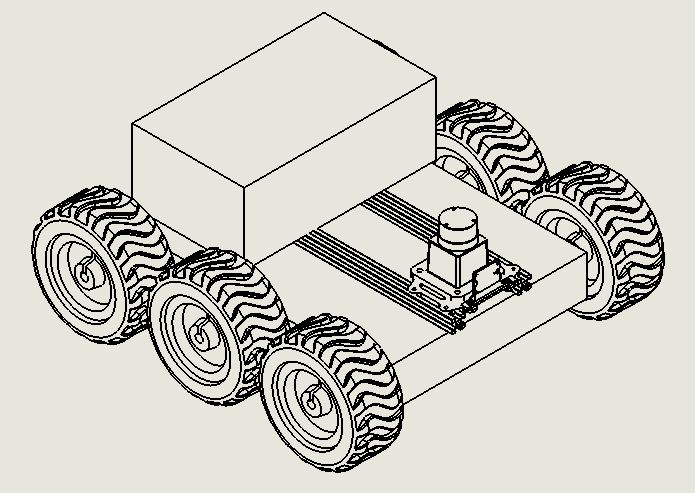
\includegraphics[width=\textwidth]{IMP}
	    \caption{Isometric view.}
	    \label{fig:IMP}
    \end{subfigure}
    \quad %add desired spacing between images, e. g. ~, \quad, \qquad, \hfill etc.
      %(or a blank line to force the subfigure onto a new line)
    \begin{subfigure}[b]{0.3\textwidth}
        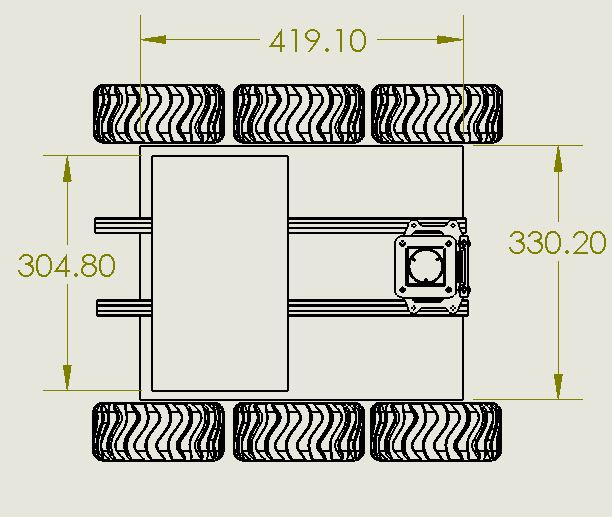
\includegraphics[width=\textwidth]{IMPtop}
        \caption{Top view.}
        \label{fig:IMPtop}
    \end{subfigure}%
    \quad %add desired spacing between images, e. g. ~, \quad, \qquad, \hfill etc.
      %(or a blank line to force the subfigure onto a new line)
    \begin{subfigure}[b]{0.3\textwidth}
        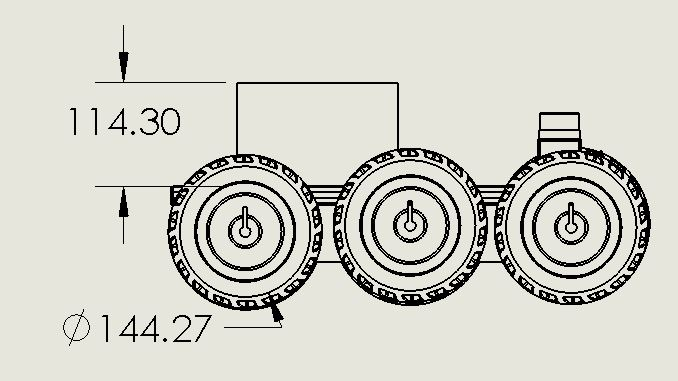
\includegraphics[width=\textwidth]{IMPside}
        \caption{Side view.}
        \label{fig:IMPside}
    \end{subfigure}%
    \caption{Dimensions of \imp.}
    \label{fig:IMPviews}
\end{figure}

Once the type of robot was decided, the next important consideration was the size. This mainly depends on the budget and the application the robot is being built for. As per the design principles stated, the primary objective is to keep the robot scalable, and equipped to carry larger payloads. So the slightly larger size of the robot will allow payloads to be attached in the future. The dimensions of the robot are shown in Figure~\ref{fig:IMPviews}. The chassis is designed to be light weight but structurally sound so as to allow larger payload capability. For this purpose the material of choice is aluminum. It has the lightness offered by plastics and none of the structural weaknesses exhibited by it. The chassis structure itself is an hollow cuboid, but there are multiple support struts running across it's breadth to give added strength. This design allows us to minimize the weight of the chassis to about 2.2 kg. 

The guiding principle behind the design of the robot was versatility. Therefore, the wheels were chosen to be made of rubber with a offset-V tread to have sufficient friction to traverse both indoor and outdoor environments. The wheel size was decided based on the size of platform. The number of wheels were chosen based on both stability, control and sensing requirement. The four outer wheels were decided to be powered using a DC geared motor so that sufficient torque can be generated to allow the robot to have a small turning radius. Putting the encoders on the same wheels will give errors in odometry when there is slipping of the wheels because of friction loss which is a common occurrence on gravel in outdoor environments and on smooth floors indoors. Due to this the two middle wheels were added, which are used for odometry. Since it is only the movement of the robot which will cause the middle wheels to turn, it gives a better estimate of the path followed by the robot which gives a huge benefit, for autonomous applications. 

Once the basic platform is designed, the choice of motors and battery is a combined decision, the torque capacity of the motors depend mainly on the weight of the payload that is to be carried by the robot. More the torque capacity the current drawn is more hence for the same run time a larger battery is needed which in turn increases the weight of the payload. For example, in a previous version, the same platform had a 24V nickel-metal hydride(Ni-MH) battery and DC geared motors with a rated torque of 1.4 kgf-cm. Since a typical Ni-Mh battery has a specific energy of 20-120 Wh/kg, a battery which had an energy rating of 4500 mAh, weighed around 1.5 kg. With this configuration, it was found that the motors were not strong enough to turn just the platform itself with a reasonable turn radius. This was due to a combination of both the large weight of the battery and the low torque of the motor. 

Both the batteries and the motors were then upgraded, to enable the platform to carry not only it's own weight but also additional sensor and computational payload. Ni-MH batteries were replaced by high specific energy lithium polymer(LiPo) batteries. These batteries typically have a specific energy of 100-265 Wh/kg. The battery used on IMP with 2500mAh, weighs around 0.4 kg. Even though the battery capacity has reduced by a factor of 2, the weight reducing by a factor of 3 compensated for it. Also, the low weight allows further increase of the battery capacity without having to change the motors if needed. The motors currently used on the \imp have a rated load of 7.3 kgf-cm, which makes the IMP ideal for larger payloads.

%As seem in Figure~\ref{fig:IMP_color} and~\ref{fig:IMP}, the rest of the components on IMP are attached using an aluminum channel as shown in Figure~\ref{fig:mounting} and not welded. This allows for easy switching during further expansion. The Sensors are also mounted using 3D printed modular mounts as in Figure~\ref{fig:modular_hokuyoBase}.
%
%\begin{figure}
%    \centering
%    \begin{subfigure}[b]{0.4\textwidth}
%		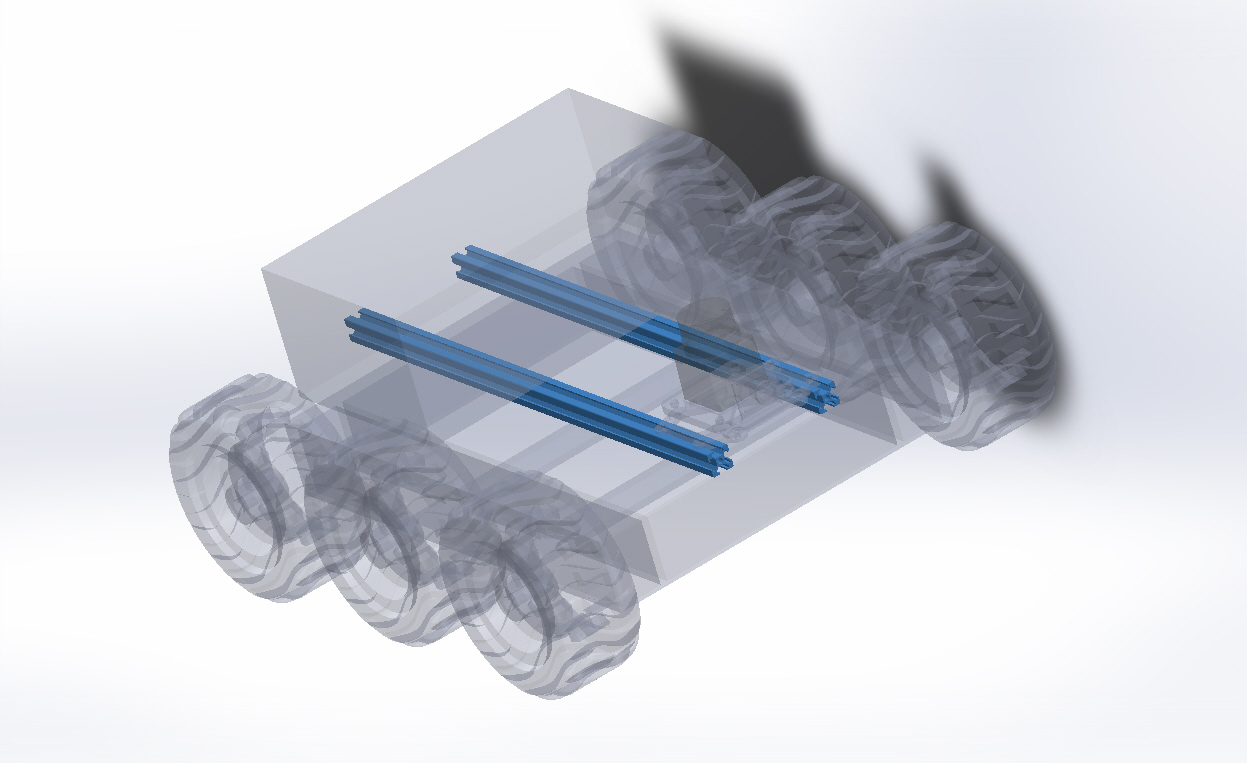
\includegraphics[width=\textwidth]{beams}
%		\caption{Mounting rails on IMP}
%		\label{fig:mounting}
%    \end{subfigure}
%    \qquad %add desired spacing between images, e. g. ~, \quad, \qquad, \hfill etc.
%      %(or a blank line to force the subfigure onto a new line)
%    \begin{subfigure}[b]{0.4\textwidth}
%        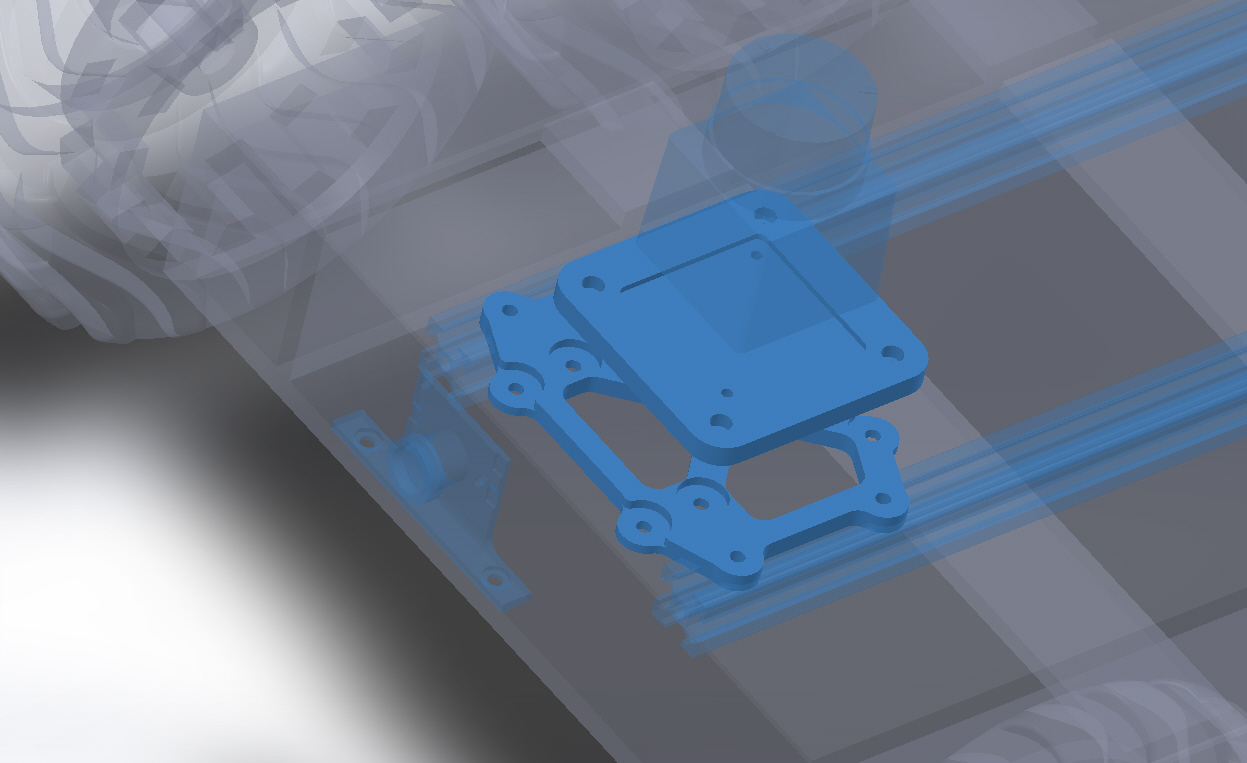
\includegraphics[width=\textwidth]{modular_hokuyoBase}
%        \caption{Mounting plates for sensors}
%        \label{fig:modular_hokuyoBase}
%    \end{subfigure}
%    \caption{Modular design of IMP}
%    \label{fig: Modular}
%\end{figure}

\section{Electrical Design}

The electrical design is guided by the same principles of Scalability for autonomy, and flexibility. The major computational and sensory payloads on the IMP are:

\begin{itemize}
\item 	Dual processor AutoPilot unit with a 12-axis inertial measurement unit
\item  	ODROID-XU Computer
\item 	MA 3 Miniature Absolute Magnetic Shaft Encoders
\item  	Leopard Imaging 5 MP camera
\item  	Hokuyo-URG
\item	TP-Link Nano Wireless Module
\item  	XBEE Wireless radio
\end{itemize}
\begin{figure}
\centering
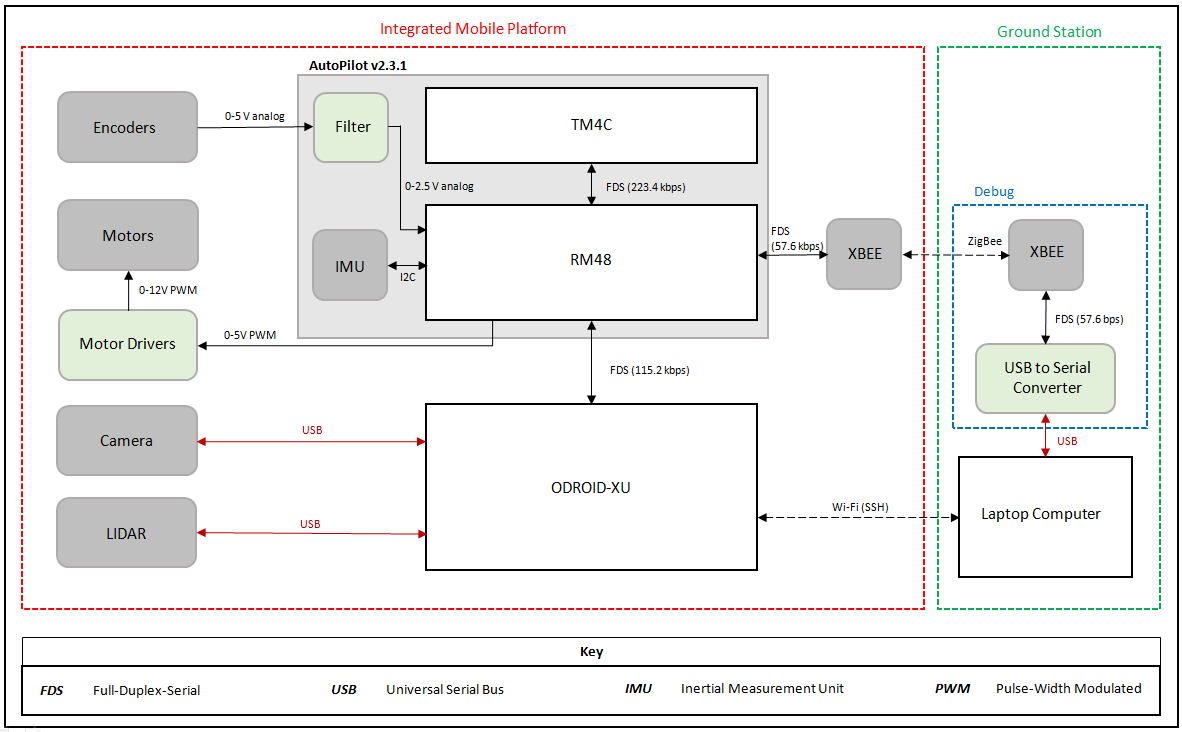
\includegraphics[width = \textwidth]{system_diagram}
\caption{System diagram of \imp.}
\label{fig:system_digram}
\end{figure}
\subsection{Device purpose and descriptions}
\begin{figure}
\centering
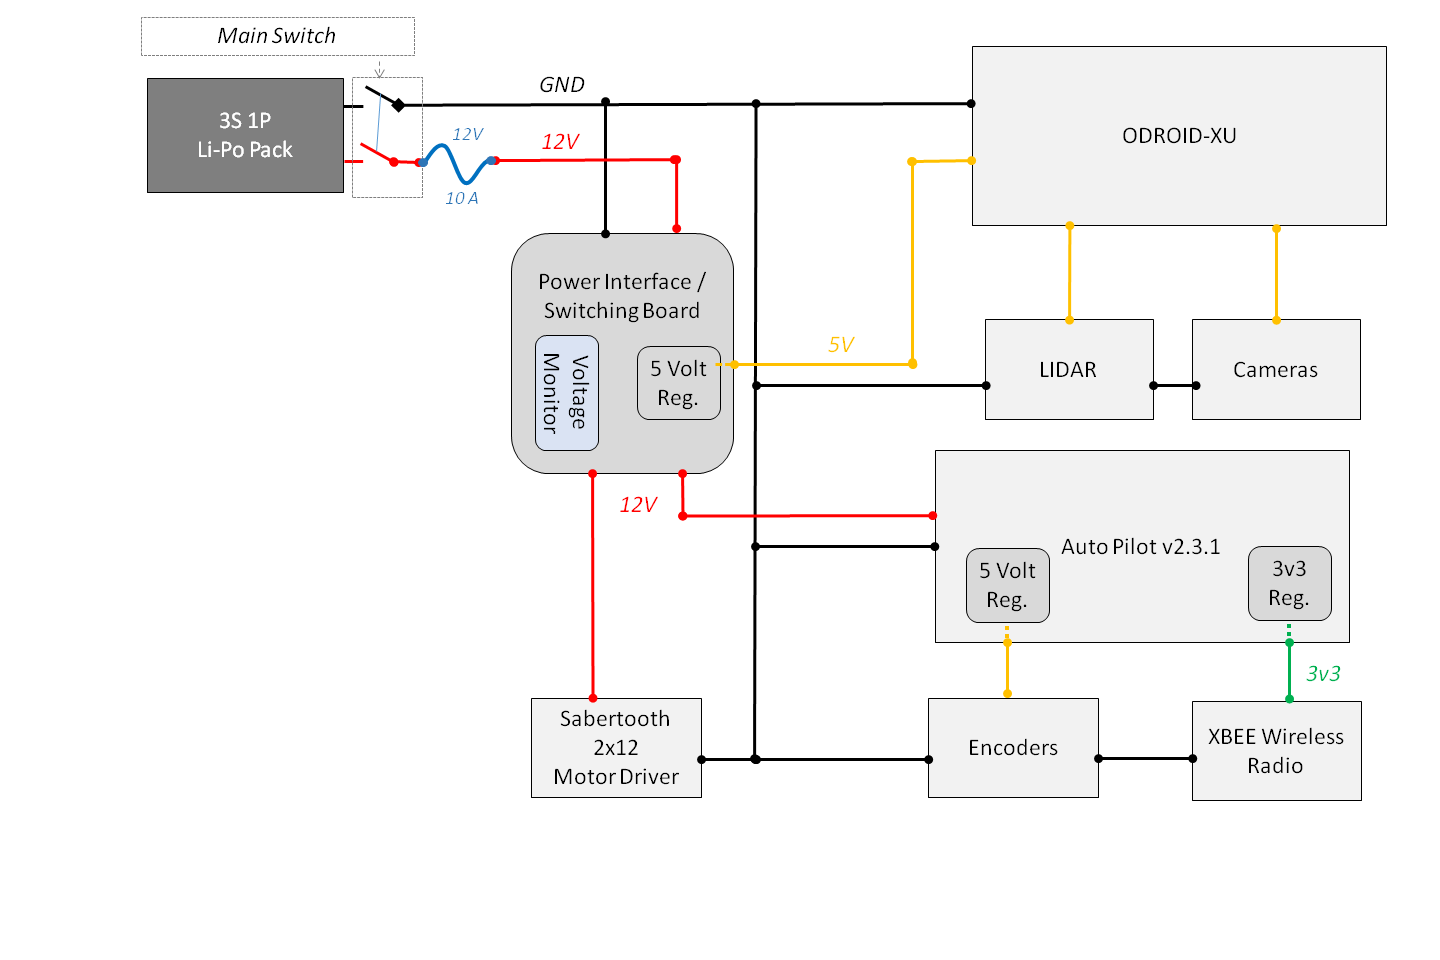
\includegraphics[width = \textwidth]{power_diagram}
\caption{\imp Power routing diagram.}
\label{fig:power_diagram}
\end{figure}

\subsubsection{AutoPilot}

The AutoPilot is a dual processor unit that is equipped for low level control algorithms as well to act as an input/output interface for the robot. The AutoPilot consists of two processing units: a TM4C and RM48 micro-controller (MCU), which operate at 80 MHz and 220 MHz, respectively. These processors can communicate with each other either over UART or Controller Area Network(CAN). One UART of the RM48 MCU is also connected to an on-board computer, an ODROID-XU through a level translator circuit. The AutoPilot is powered via an external 12 V supply. This AutoPilot unit includes a 12-axis inertial measurement unit (IMU) which consists of two, 3-axis accelerometers, one 3-axis rate gyro, and a 3-axis magnetometer unit. Additionally, the AutoPilot includes humidity and temperature sensors and receives GPS signals. 

The AutoPilot being a versatile device can be used for a large number of purposes depending on the implementation. A part of the autonomy algorithm can be off loaded to the AutoPilot, or low level control algorithms such as PID can be implemented on it. It is currently implemented as an I/o processing unit. It interfaces with the encoders, the motor driver while acquiring measurements from the IMU.

\subsubsection{ODROID XU}

The ODROID is the on-board computer. It plays a major part if the IMP is used for real time autonomous navigation. It is equipped with Samsung Exynos5422 Cortex™-A15 2.0Ghz quad core and Cortex™-A7 quad core CPUs. It has 2Gbyte LPDDR3 RAM capable of operating at 933MHz and several USB 2 and USB 3 ports for interfacing. With these features it can run considerably powerful algorithms for \slam and also path planning and decision making. It is the higher level controller of the robot. It is powered by a seperate 5V regulator as shown in Figure~\ref{fig:power_diagram}.

\subsubsection{Encoders}
\begin{figure}[h]
\centering
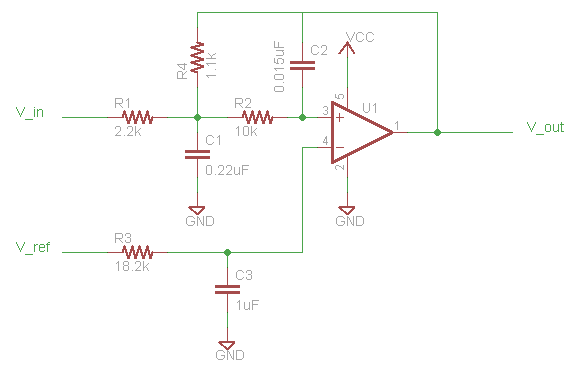
\includegraphics[width=0.4\textwidth]{low_pass}
\caption{Low pass filter for encoder input.}
\label{fig:low_pass}
\end{figure}
The magnetic shaft encoders give the absolute position of the wheel. From the perspective of a device interfacing with it, it can be modeled as a potentiometer. It gives 0-5V analog output corresponding to the angle the wheel is at currently. So while the wheel is continuously turning, the value rises from 0 to 5 volts and then suddenly drops to 0. Therefore, to calculate movement the encoder signal has to be first stored in an accumulator and then differentiated. The signal is considerably free of noise and performs reasonably well for dead reckoning, it has some high frequency noise that needs to be filtered out. So the analog signal is first passed through an active low pass filter of 950 Hz which is shown in Figure~\ref{fig:low_pass}. A Digital to Analog Converter(DAC) is used to be able to set the reference voltage without having to change the hardware. Both the filter circuit and the DAC is inbuilt into the AutoPilot.

\subsubsection{Camera}

The major advantage of an on-board camera is that it can act both as an exteroceptive sensor as well as a proprioceptive sensor. The camera can be used for sensing features in the environment. It can also be used for visual odometry which gives an estimate of the robot's pose.

The Leopard imaging Camera, captures 5 mega pixel HD images at speeds up to 30 frames per second. It can has a $ 72^\circ $ horizontal field of view, and $ 30^\circ $ vertical. It has a simple USB interface and it's data is read into the ODROID.

\subsubsection{LIDAR}
When picking a LIDAR, first the choice needs to be made between using 2D or 3D LIDARs. 3D LIDARs while having numerous advantages, it's high cost limits the application of the robot. It is more practical to have a 2D LIDAR initially with scope for further expansion into 3D. A really simple way to implement 2D LIDAR is to have a single range finder and mount it on a rotating platform. That way the cost can be reduced but the resolution and scanning speed are adversely affected. An earlier iteration of IMP, used a Piccolo Laser Scanner, which had an inexpensive laser range finder being rotated at around 15 Hz. The range finder itself, was based on beam deviation rather than \textit{Time of Flight} which made it slightly inaccurate. 

The current LIDAR used is the Hokuyo URG-04LX Scanning Laser Range Finder which has a low scanning of 100 ms/scan, and is accurate up to 2 mm. It has a $ 240^\circ $ field of view and can detect from 20 mm to 5600 mm. It is read through a USB port into the ODROID. With this LIDAR, the robot has the capability of sensing the environment to a largely accurate extant.

\subsubsection{Communication Modules}
The primary channel of communication is the Wi-Fi module, TP-Link Nano. It has a speed of 150 Mbps and is configured in \textit{AP Router} mode. This is done so that IMP can host its own Wi-Fi to which any ground station that needs to interact with it can connect to it directly. This is advantageous when IMP is to be used outdoors and there is no existing Wi-Fi networks available. 

Another interface is the XBee connected directly to the AutoPilot through an UART port. This can be used if the AutoPilot is to be commanded directly for tele-operation without using the ODROID. In the current configuration it is used as a Debug port so that the status of the AutoPilot can be checked whenever needed. 
\section{Software Design for data collection}
The Autopilot having a precise Real Time Interrupt module in the RM48, maintains timebase for the whole process. It's interrupts are set in a half millisecond cycles. Every millisecond it reads the encoders and updates an accumulator. The IMU are read every 5 ms. Both the encoders and the IMUs are logged on the SD card at a rate of 80Hz. Every 10 ms, the latest accumulator and IMU readings are sent to the ODROID. 

The ODROID, parses the data sent by the AutoPilot. Based on the standard time base, at the rate of 5 Hz, the on-board camera and the LIDAR data is acquired. All the collected data is stored in the file system of the Odroid. These files are then transfered through SSH to the ground station. The ODROID program itself is started and controlled over Wi-Fi, through which the user commands are transmitted. 

\section{Encoder Based Odometry for State Estimate}

The encoders attached on the two passive wheels give an estimate of the robot's movement in each time step. The function used to calculate the robot's movement from the encoder data is the motion model of the robot and is used for equation~\ref{eq:EKF_1} in section~\ref{sec:EKF}. Since this robot has only 3 degrees of freedom, the state vector, $ x \in \Re^3 $ and is defined as $ x = [x,y,\theta]^T $ where $ x $ and $ y $ give the position of the robot from an arbitrary fixed point in inertial frame of reference. 

\subsection{Motion model and the corresponding differentials}

To estimate the motion model, first left and right wheel movement is converted into distances traveled through a linear mapping using the known radius of the wheels. These values are represented by $ u = [ l, r ]^T $. The equations are better implemented as a piecewise function. The two cases of when the robot is estimated to be going straight or to be turning is considered separately. This decision is made by observing the distance traveled by the left and right wheels. If they are exactly the same, the robot is going straight and the motion model is given by equations~\ref{eq:Enc_1}. 

If $ r = l $:
\begin{equation}
\label{eq:Enc_1}
	\begin{bmatrix}
		\hat{x}^-\\\hat{y}^-\\\hat{\theta}^-
	\end{bmatrix}_k
	=
	\begin{bmatrix}
		\hat{x}\\\hat{y}\\\hat{\theta}
	\end{bmatrix}_{k-1}
	+
	\begin{bmatrix}
		l.\cos(\hat{\theta}_{k-1})\\
		l.\sin(\hat{\theta}_{k-1})\\
		0
	\end{bmatrix}
\end{equation}	

If not, then the robot is turning, and equations~\ref{eq:Enc_2} and~\ref{eq:Enc_3} are used. Where $ R,\alpha $ and $ w $ are as shown in Figure~\ref{fig:Enc_1}
			
\begin{figure}
\centering
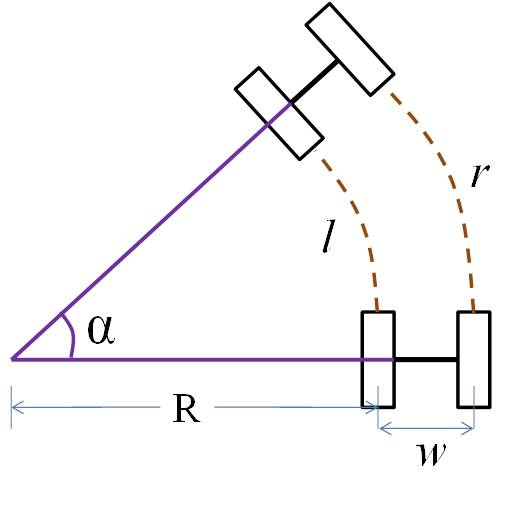
\includegraphics[width=0.3\textwidth,height=0.3\textheight]{differential_turning}
\caption{Motion model of differential drive platform.}
\label{fig:Enc_1}
\end{figure}
If $ r \neq l $:
\begin{equation}
\label{eq:Enc_2}
	\alpha= \frac{r-l}{w}
\qquad
	R=\frac{l}{\alpha}
\end{equation}
\begin{equation}
\label{eq:Enc_3}
	\begin{bmatrix}
		\hat{x}^-\\\hat{y}^-\\\hat{\theta}^-
	\end{bmatrix}_k
	=
	\begin{bmatrix}
		\hat{x}\\\hat{y}\\\hat{\theta}
	\end{bmatrix}_{k-1}
	+
	\begin{bmatrix}
		\left(R+\frac{w}{2}\right)(\sin(\hat{\theta}_{k-1}+\alpha)-\sin(\hat{\theta}_{k-1}))\\
		\left(R+\frac{w}{2}\right)(-\cos(\hat{\theta}_{k-1}+\alpha)-\cos(\hat{\theta}_{k-1}))\\
		\alpha
	\end{bmatrix}
\end{equation}

In general for ease of representation this motion model is referred to only by $ f $. 
\begin{equation}[h!]
\label{eq:Enc_4}
\hat{x}^-_k = f(\hat{x}_{k-1},u_k)
\end{equation}

Once the motion model is known, it is necessary to find it's Jacobian with respect to the state. Since both the motion model $ f $ and the state have 3 dimensions the Jacobian will be a $ 3\times 3 $ matrix given by~\ref{eq:Enc_5}. 

\begin{equation}
\label{eq:Enc_5}
A = \frac{\partial f}{\partial x} = 
\begin{bmatrix}
\frac{\partial f_1}{\partial x} & \frac{\partial f_1}{\partial y} & \frac{\partial f_1}{\partial z} \\
\frac{\partial f_2}{\partial x} & \frac{\partial f_2}{\partial y} & \frac{\partial f_2}{\partial z} \\
\frac{\partial f_3}{\partial x} & \frac{\partial f_3}{\partial y} & \frac{\partial f_3}{\partial z}
\end{bmatrix}
\end{equation}

Since the motion model is piecewise, it's Jacobian also calculated in two parts by differentiating the respective equations~\ref{eq:Enc_1} and~\ref{eq:Enc_3}.

If $ r = l $:
\begin{equation}
\label{eq:Enc_6}
A = 
\begin{bmatrix}
1 & 0 & -l\sin\theta\\
0 & 1 & -l\cos\theta\\
0 & 0 & 1
\end{bmatrix}
\end{equation}

If $ r \neq l $
\begin{equation}
\label{eq:Enc_7}
A = 
\begin{bmatrix}
1 & 0 & (R+\frac{w}{2})(\cos(\theta+\alpha)-\cos\theta)\\
0 & 1 & (R+\frac{w}{2})(\sin(\theta+\alpha)-\sin\theta)\\
0 & 0 & 1
\end{bmatrix}
\end{equation}

Where $ R,w $ and $ \alpha $ are according to equation~\ref{eq:Enc_2} and Figure~\ref{fig:Enc_1}

Next the motion model is differentiated with respect to the noise. Here the process noise is assumed to be essentially due to the noise in encoder measurement and it is additive in nature. Hence it is possible to know the variance of the movement with respect to noise by differentiating the motion model with respect to the encoder measurements $ l $ and $ r $. Since this is of dimension 2, the noise covariance matrix W will be of dimension $ 3\times 2 $ given by equation~\ref{eq:Enc_8}.

\begin{equation}
\label{eq:Enc_8}
W = \frac{\partial f}{\partial (u+w)} = \frac{\partial f}{\partial (u)} =
\begin{bmatrix}
\frac{\partial f_1}{\partial l} & \frac{\partial f_1}{\partial r}\\
\frac{\partial f_2}{\partial l} & \frac{\partial f_2}{\partial r}\\
\frac{\partial f_3}{\partial l} & \frac{\partial f_3}{\partial r}
\end{bmatrix} 
\end{equation}
Each of the individual terms are then calculated independently.
\begin{subequations}
If $ r=l $:
	\begin{align}
		\frac{\partial f_1}{\partial l} &= \frac{1}{2}(\cos\theta+\frac{l}{w}\sin\theta)\\
		\frac{\partial f_2}{\partial l} &= \frac{1}{2}(\sin\theta-\frac{l}{w}\cos\theta)\\
		\frac{\partial f_1}{\partial r} &= \frac{1}{2}(-\frac{l}{w}\sin\theta+\cos\theta)\\
		\frac{\partial f_2}{\partial r} &= \frac{1}{2}(\frac{l}{w}\cos\theta+\sin\theta)\\
		\frac{\partial f_3}{\partial l} &= -\frac{1}{w} \quad \frac{\partial f_3}{\partial r} = \frac{1}{w}
	\end{align}
\end{subequations}

\begin{subequations}
If $ r\neq l $:
	\begin{align}
		\frac{\partial f_1}{\partial l} &= \frac{wr}{(r-l)^2}(\sin\theta'-\sin\theta)-\frac{r+l}{2(r-l)}\cos\theta'\\
		\frac{\partial f_2}{\partial l} &= \frac{wr}{(r-l)^2}(-\cos\theta'+\cos\theta)-\frac{r+l}{2(r-l)}\sin\theta'\\
		\frac{\partial f_1}{\partial r} &= \frac{-wr}{(r-l)^2}(\sin\theta'-\sin\theta)+\frac{r+l}{2(r-l)}\cos\theta'\\
		\frac{\partial f_2}{\partial r} &= \frac{wr}{(r-l)^2}(-\cos\theta'+\cos\theta)-\frac{r+l}{2(r-l)}\sin\theta'\\
		\frac{\partial f_3}{\partial l} &= -\frac{1}{w} \quad \frac{\partial f_3}{\partial r} = \frac{1}{w}
	\end{align}
\end{subequations}

Where, $ \theta'=\theta+\alpha $ and $ R,w $ and $ \alpha $ are as per Figure~\ref{fig:Enc_1}. Once the Jacobian is calculated, the last component needed for the estimation according to equation~\ref{eq:EKF_4} is the Process noise covariance $ Q $. This has to contain some information about the amount the noise in each time step. Since all noise is assumed to be only sensor measurement noise, a diagonal matrix with the error in each encoder is chosen as the covariance as in equation~\ref{eq:Enc_9}.

\begin{equation}
\label{eq:Enc_9}
Q = 
\begin{bmatrix}
\sigma_l^2 & 0\\
0 & \sigma_r^2
\end{bmatrix}
\end{equation}

\subsection{Limitations of odometry based estimation}

One of the primary limitation of estimating a robot's position solely on odometry is that, over a long time, the error accumulates and results in the estimate being very far from the actual position of the robot. Also every real world encoder has a component of noise which accumulates over time. In indoor environments, there is a good chance of wheel slippage especially during turns making it hard to accurately reconstruct a turn. Another drawback is that if the encoder wheels are not fully lubricated and free to move, any wheel might stop moving with the robot and skid instead. This will result in the reconstruction seeing a turn, whereas the robot itself might have been moving straight. To correct these, is the major motivation in any SLAM algorithm. 
